\documentclass[10pt]{article}
\usepackage[T1]{fontenc}
\usepackage[utf8]{inputenc}
\usepackage{lmodern}
\usepackage[a4paper,margin=18mm]{geometry}
\usepackage{amsmath,amssymb,mathtools}
\usepackage{microtype}
\usepackage{graphicx}
\usepackage[hidelinks]{hyperref}
\pdfinfoomitdate=1
\pdfsuppressptexinfo=-1
\pdftrailerid{<474f5244414e2d54484554412d44452d31><474f5244414e2d54484554412d44452d31>}
\pagestyle{empty}
\setlength{\parindent}{0pt}
\setlength{\parskip}{0.28em}
\setlength{\abovedisplayskip}{0.45em}
\setlength{\belowdisplayskip}{0.45em}
\newcommand{\dd}{\partial}
\newcommand{\sourceanchor}[1]{\hypertarget{source-#1}{}}
\allowdisplaybreaks
\hypersetup{pdftitle={Ueber die Transformation der Thetafunctionen - German diplomatic transcription},pdfauthor={Paul Gordan},pdfsubject={Source-faithful diplomatic transcription, 1863}}
\begin{document}
\small

% Source: Google Books page-image witnesses PA1-PA20, Gordan 1863 theta transformation.
% Non-authorial Google watermark and PA2 library stamp/digitization debris are not transcribed in the authorial text.
\sourceanchor{PA01}
\begin{center}
{\Large UEBER DIE TRANSFORMATION}\\[0.7em]
{\normalsize DER}\\[0.7em]
{\large \(\Theta\)FUNKTIONEN.}\\[1.2em]

\includegraphics[width=0.15\linewidth]{assets/PA01_title_divider_presentation_4x.png}\\[1.4em]
{\large INAUGURALABHANDLUNG}\\[0.7em]
{\normalsize DER PHILOSOPHISCHEN FACULTÄT}\\[0.55em]
{\normalsize DER}\\[0.55em]
{\normalsize LUDWIGS-UNIVERSITÄT GIESSEN}\\[0.75em]
{\large ZUR ERLANGUNG DER VENIA LEGENDI}\\[0.75em]
{\normalsize VORGELEGT}\\[0.55em]
{\normalsize VON}\\[0.55em]
{\large PAUL GORDAN,}\\[-0.15em]
{\scriptsize Dr. phil.}\\[2.4em]
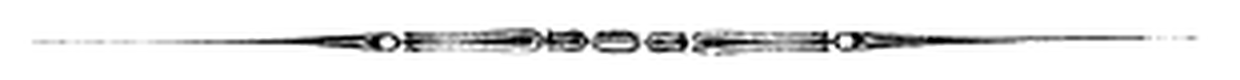
\includegraphics[width=0.52\linewidth]{assets/PA01_title_ornament_presentation_4x.png}\\[0.8em]
{\normalsize GIESSEN, 1863.}\\[-0.1em]
{\normalsize DRUCK VON WILHELM KELLER.}
\end{center}

\sourceanchor{PA02}% blank/copy-specific unit; no authorial text
\sourceanchor{PA03}
\subsection*{\S. 1.}
Die Reihe:
\[
\sum_{\alpha=-\infty}^{\infty} e^{a\alpha^{2}+2ib\alpha}
\]
ist für alle (reellen und imaginären) endlichen Werthe der Variabeln \(b\) convergent, vorausgesetzt, daß der reelle Theil der Größe \(a\) wesentlich negativ ist; man nennt sie eine \(\Theta\)Funktion und bezeichnet sie mit: \(\Theta(a,b)\); die Größen \(a\) und \(b\), von denen sie abhängt, sollen die Namen Modulus und Argument führen.

\subsection*{\S. 2.}
Die wichtigsten Eigenschaften der \(\Theta\)Functionen bestehen in folgenden Relationen, deren Beweis wir hier übergehen können.

Bedeutet \(n\) irgend eine ganze Zahl, dann ist:
\begin{align*}
1.\quad& \Theta(a,b+n\pi)=\Theta(a,b)\\
2.\quad& e^{-\frac{b^{2}}{a}}\Theta(a,b)=e^{-\frac{(b+nia)^{2}}{a}}\Theta(a,b+nia)\\
3.\quad& \Theta(a,b)=e^{n^{2}a-2nib}\Theta(a,b+nia)\\
4.\quad& \Theta(a+2n\pi i,b)=\Theta(a,b)\\
5.\quad& \Theta\!\left(a+n\pi i,b\pm \frac{n\pi}{2}\right)=\Theta(a,b)\\
6.\quad& \frac{\dd^{2}\Theta(a,b)}{\dd b^{2}}+4\frac{\dd\Theta(a,b)}{\dd a}=0.
\end{align*}

\subsection*{\S. 3.}
Durch die Gleichungen 1) und 3) wird eine \(\Theta\)Function vollständig definirt. Das heißt: Genügt die synektische Funktion \(f(b)\) den Relationen:
\[
f(b+n\pi)=f(b)
\]
\[
f(b)=e^{n^{2}a-2ibn}f(b+nia)
\]
dann ist sie bis auf einen constanten Faktor gleich \(\Theta(a,b)\).

\sourceanchor{PA04}
\begin{center}Beweis.\end{center}
Die 1. Relation lehrt uns, daß die Funktion \(f\) in eine Reihe von der Form:
\[
f(b)=\sum_{\alpha=-\infty}^{\infty} e^{x_{\alpha}+\alpha ib}
\]
entwickelt werden kann; mit Hülfe der letzteren Formel kann man Beziehungen zwischen den Constanten \(x\) aufstellen.

Da die Reihen:
\[
f(b)=\sum_{\alpha=-\infty}^{\infty}e^{x_{\alpha}+2ib\alpha}
\]
und:
\[
e^{an^{2}-2ibn}f(b+nia)=\sum_{\beta=-\infty}^{\infty}e^{x_{\beta}+2ib\beta+an^{2}-2ibn-2\beta an}
\]
identisch sind, müssen die Coëfficienten gleichhoher Potenzen von \(e^{ib}\) in beiden Reihen übereinstimmen.

Setzt man daher:
\[
\beta=n+\alpha
\]
dann muß:
\[
x_{\alpha}=x_{\beta}-2\beta an+an^{2}
\]
sein.

Diese Relation hat stets Geltung, welche ganzen Zahlen \(\alpha\) und \(n\) auch sein mögen; es ist daher gestattet für \(\alpha\) 0, für \(n\) \(\alpha\) und für \(\beta\) \(\alpha\) zu setzen; dann wird:
\[
x_{\alpha}=x_{0}+a\alpha^{2}
\]
und wenn wir diesen Werth in unsere Gleichung substituiren:
\[
f(b)=\sum_{\alpha=-\infty}^{\infty}e^{a\alpha^{2}+2ib\alpha+x_{0}}.
\]

\subsection*{\S. 4.}
Der so eben hergeleitete Satz rührt von Jacobi her und ist von demselben in fund. pag. 176 auf ähnliche Art wie hier bewiesen worden; er ist jedoch einer wichtigen Erweiterung fähig.

Genügt die synektische Funktion \(f(b)\) den Relationen:
\[
f(b+\pi)=f(b)
\]
\[
f(b)=e^{c-2nib}f(b+ia)
\]
in denen \(c\) eine Constante und \(n\) eine gegebene Zahl bedeutet; dann kann man \(f(b)\) als eine Summe von \(n\) \(\Theta\)Functionen bestimmen, deren jede eine Potenz von \(e^{ib}\) und eine willkürliche Constante zum Factor hat.

\begin{center}Beweis.\end{center}
Die Relation:
\[
f(b+\pi)=f(b)
\]
lehrt uns wieder, daß man die Funktion \(f(b)\) in eine Reihe von der Form:
\sourceanchor{PA05}
\begin{equation*}
 f(b)=\sum_{\alpha=-\infty}^{\infty}e^{x_{\alpha}+2ib\alpha}
\tag{1}
\end{equation*}
entwickeln kann, während wir die Formel:
\[
f(b)=e^{c-2nib}f(b+ia)
\]
dazu benutzen, um Beziehungs-Gleichungen zwischen den Constanten \(x\) aufzustellen.

Aus der Identität der beiden Reihen:
\[
f(b)=\sum_{\alpha=-\infty}^{\infty}e^{x_{\alpha}+2ib\alpha}
\]
und:
\[
e^{c-2nib}f(b+ia)=\sum_{\beta=-\infty}^{\infty}e^{x_{\beta}+2ib\beta-2ibn+c-2\beta a}
\]
folgt, daß, wenn man:
\[
\beta=n+\alpha
\]
setzt:
\[
x_{\alpha}=x_{\beta}+c-2\beta a=x_{\alpha+n}+c-2an-2a\alpha.
\]
Aus dieser Gleichung ersehen wir, daß die \(n\) ersten der Constanten \(x\) willkürlich sind, die übrigen \(x\) indeß aus diesen berechnet werden können.

Wir wollen nun die Reihe, in welche wir \(f(b)\) entwickelt haben, in eine Doppel-Reihe verwandeln und setzen zu dem Ende:
\[
\alpha=n\gamma+\delta.
\]
Damit nun \(\alpha\) alle ganzzahligen Werthe von \(-\infty\) bis \(+\infty\) annehme, müssen wir bei der Summation für \(\gamma\) alle Zahlen von \(-\infty\) bis \(+\infty\) setzen, während wir gleichzeitig über die Werthe 0 bis \(n-1\) von \(\delta\) summiren.

Es ergeben sich somit die beiden Formeln:
\begin{align}
 f(b)&=\sum_{\delta=0}^{n-1}e^{2ib\delta}\sum_{\gamma=-\infty}^{\infty}e^{x_{\gamma n+\delta}+2ibn\gamma} \tag{2}\\
 x_{\gamma n+\delta}&=x_{(\gamma+1)n+\delta}+c-2a\delta-2an(\gamma+1). \tag{3}
\end{align}
Lassen wir in Formel (3) \(\gamma\) alle Werthe von 0 bis \(\gamma-1\) annehmen, dann erhalten wir folgendes System Gleichungen:
\begin{align*}
 x_{n+\delta}&=x_{\delta}-c+2a\delta+2an\\
 x_{2n+\delta}&=x_{n+\delta}-c+2a\delta+4an\\
 x_{3n+\delta}&=x_{2n+\delta}-c+2a\delta+6an\\
 &\hspace{2em}\cdots\cdots\cdots\cdots\cdots\cdots\\
 x_{\gamma n+\delta}&=x_{(\gamma-1)n+\delta}-c+2a\delta+2\gamma an
\end{align*}
und wenn wir alle diese Formeln addiren:
\[
x_{\gamma n+\delta}=x_{\delta}-\gamma c+2\gamma a\delta+an(\gamma+1)\gamma.
\]
Tragen wir diesen Werth in unsere Doppel-Reihe (2) ein, erhalten wir endlich:
\begin{align*}
 f(b)&=\sum_{\delta=0}^{n-1}e^{2ib\delta+x_{\delta}}\sum_{\gamma=-\infty}^{\infty}e^{an\gamma^{2}+an\gamma-\gamma c+2\gamma a\delta+2ibn\gamma}\\
 &=\sum_{\delta=0}^{n-1}C_{\delta}e^{2ib\delta}\Theta\!\left(an,bn-\frac{ian}{2}+\frac{ic}{2}-ia\delta\right).
\end{align*}

\sourceanchor{PA06}
\subsection*{\S. 5.}
Aus den Formeln 1. und 3. läßt sich leicht folgern, daß die Funktion:
\[
f(b)=e^{\frac{b^{2}}{a}}\Theta\!\left(\frac{\pi^{2}}{a},\frac{ib\pi}{a}\right)
\]
den Relationen genügt:
\[
f(b+\pi)=f(b)
\]
\[
f(b+ia)=e^{-a+2ib}f(b).
\]
Nach dem im \S. 3 bewiesenen Satz ist also:
\[
f(b)=C\Theta(a,b)
\]
und mithin identisch:
\begin{equation*}
\Theta(a,b)=C e^{\frac{b^{2}}{a}}\Theta\!\left(\frac{\pi^{2}}{a},\frac{ib\pi}{a}\right)
\tag{1}
\end{equation*}
in welcher Formel \(C\) von \(b\) unabhängig, also eine noch zu bestimmende Funktion von dem Modulus \(a\) bedeutet.

\subsection*{\S. 6.}
Die Bestimmung von \(C\) läßt sich auf folgende Weise bewerkstelligen. -- Substituirt man in der Formel 6.
\[
\frac{\dd^{2}\Theta(a,b)}{\dd b^{2}}+4\frac{\dd\Theta(a,b)}{\dd a}=0
\]
für \(\Theta(a,b)\) seinen Werth aus Gleichung (1), dann erhält man:
\begin{align*}
& C e^{\frac{b^{2}}{a}}\Biggl\{\Theta\!\left(\frac{\pi^{2}}{a},\frac{ib\pi}{a}\right)\!\left(\frac{2}{a}+\frac{4b^{2}}{a^{2}}\right)
 +2\frac{\dd\Theta\!\left(\frac{\pi^{2}}{a},\frac{ib\pi}{a}\right)}{\dd\left(\frac{ib\pi}{a}\right)}\cdot\frac{i\pi}{a}\cdot\frac{2b}{a}
 -\frac{\dd^{2}\Theta\!\left(\frac{\pi^{2}}{a},\frac{ib\pi}{a}\right)}{\dd\left(\frac{ib\pi}{a}\right)^{2}}\cdot\frac{4\pi^{2}}{a^{2}}\Biggr\}\\
&\quad +4C e^{\frac{b^{2}}{a}}\Biggl\{\Theta\!\left(\frac{\pi^{2}}{a},\frac{ib\pi}{a}\right)\cdot\left(-\frac{b^{2}}{a^{2}}\right)
-\frac{\dd\Theta\!\left(\frac{\pi^{2}}{a},\frac{ib\pi}{a}\right)}{\dd\left(\frac{ib\pi}{a}\right)}\cdot\frac{ib\pi}{a^{2}}
-\frac{\dd\Theta\!\left(\frac{\pi^{2}}{a},\frac{ib\pi}{a}\right)}{\dd\left(\frac{\pi^{2}}{a}\right)}\cdot\frac{\pi^{2}}{a^{2}}\Biggr\}\\
&\quad +4\frac{\dd C}{\dd a}e^{\frac{b^{2}}{a}}\Theta\!\left(\frac{\pi^{2}}{a},\frac{ib\pi}{a}\right)=0.
\end{align*}
Da nun nach Formel 6:
\[
\frac{\dd^{2}\Theta\!\left(\frac{\pi^{2}}{a},\frac{ib\pi}{a}\right)}{\dd\left(\frac{ib\pi}{a}\right)^{2}}+4\frac{\dd\Theta\!\left(\frac{\pi^{2}}{a},\frac{ib\pi}{a}\right)}{\dd\left(\frac{\pi^{2}}{a}\right)}=0
\]
so wird:
\[
\frac{C}{a}+2\frac{\dd C}{\dd a}=0,
\quad\text{also}\quad
C=\sqrt{\frac{c}{a}}
\]
sein, wo \(c\) nun sowohl von \(b\) als auch von \(a\) unabhängig ist.

\sourceanchor{PA07}
Trägt man für \(C\) seinen so eben gefundenen Werth in Gleichung (1) ein, dann ergibt sich:
\[
\Theta(a,b)=\sqrt{\frac{c}{a}}e^{\frac{b^{2}}{a}}\Theta\!\left(\frac{\pi^{2}}{a},\frac{ib\pi}{a}\right).
\]
Die Constante \(c\) läßt sich dadurch bestimmen, daß man in dieser Formel für \(b\) 0 und für \(a\) \(-\pi\) setzt.

Man erhält alsdann:
\[
\Theta(-\pi,0)=\sqrt{\frac{c}{-\pi}}\Theta(-\pi,0)
\]
also:
\[
c=-\pi
\]
und:
\begin{equation*}
\Theta(a,b)=\sqrt{\frac{-\pi}{a}}e^{\frac{b^{2}}{a}}\Theta\!\left(\frac{\pi^{2}}{a},\frac{bi\pi}{a}\right).
\tag{7.}
\end{equation*}

\subsection*{\S. 7.}
Die Quadratwurzel muß man in dieser Formel so wählen, daß ihr reeller Theil positiv ist.

\begin{center}Beweis.\end{center}
Für \(a=-\pi\) erhält die Quadratwurzel den Werth 1, für diesen Werth von \(a\) ist also der reelle Theil der Wurzel positiv.

Wäre nun für \(a=a_{1}\) der reelle Theil der Wurzel negativ, dann müßte ein Werth \(a_{2}\) zwischen \(a_{1}\) und \(-\pi\) liegen, für welchen der reelle Theil von \(\sqrt{\frac{-\pi}{a_{2}}}\) verschwände.

Dieß ist aber nicht möglich, da der reelle Theil von \(a\) stets wesentlich negativ ist (s. \S. 1.)

\subsection*{\S. 8.}
Mittelst der Formel 7. kann man erkennen, in welcher Weise sich die Funktion \(\Theta(a,b)\) der Unendlichkeit nähert, wenn der Modul von \(a\) immer mehr und mehr abnimmt.

Für kleiner werdendes \(a\) nähert sich nämlich der Werth der Funktion:
\[
\Theta\!\left(\frac{\pi^{2}}{a},0\right)=\sqrt{\frac{-a}{\pi}}\Theta(a,0)
\]
immer mehr und mehr die Einheit.

\(\Theta(a,0)\) wird daher unendlich wie
\[
\sqrt{\frac{-\pi}{a}}.
\]

\subsection*{\S. 9.}
Die Formel 7. ist in der Theorie der \(\Theta\)Functionen von großer Wichtigkeit. Jacobi hat sie, wie Rosenhein in seiner Abhandlung: \textit{sur les fonctions de deux variables et à quatre périodes} angiebt, auf eine etwas andere Weise erwiesen; wir haben hier aber diese Art des Beweises vorgezogen, weil wir die dabei angewandte Methode noch in anderer Weise verwerthen wollen.

\sourceanchor{PA08}
Es ist bei gegenwärtiger Untersuchung nämlich unsere Absicht, indem wir von Formel 7. ausgehen, zu der allgemeinsten Formel zu gelangen, durch welche eine \(\Theta\)Funktion in eine andere mit einer Exponential-Funktion multiplicirte \(\Theta\)Funktion transformirt werden kann.

\subsection*{\S. 10.}
Setzt man in Formel 7. statt \(a\) \(a+2\lambda i\pi\) und bezeichnet man die Ausdrücke:
\[
\frac{\pi^{2}}{a+2\lambda i\pi}\quad\text{und}\quad \frac{ib\pi}{a+2\lambda i\pi}
\]
mit \(a_1\) und \(b_1\), so ergiebt sich die Gleichung:
\[
\Theta(a,b)=\sqrt{i\frac{b_1}{b}}\,e^{\frac{b^{2}}{a+2\lambda i\pi}}\Theta(a_1,b_1).
\]
In ähnlicher Weise kann man:
\[
a_2=-\frac{\pi^{2}}{a_1+2\lambda_1 i\pi},\qquad
b_2=\frac{i b_1\pi}{a_1+2\lambda_1 i\pi}
\]
setzen, es wird dann:
\[
\Theta(a,b)=\sqrt{i\frac{b_2}{b_1}}\,e^{\frac{b_1^{2}}{a_1+2\lambda_1 i\pi}}\Theta(a_2,b_2).
\]
Fährt man so fort, so kommt man zu folgendem System von Gleichungen:
\begin{align*}
a_1&=\frac{\pi^{2}}{a_0+2\lambda_0 i\pi},&
 b_1&=\frac{i b_0\pi}{a_0+2\lambda_0 i\pi},&
 \Theta(a_0,b_0)&=\sqrt{i\frac{b_1}{b_0}}\,e^{\frac{b_0^{2}}{a_0+2\lambda_0 i\pi}}\Theta(a_1,b_1),\\
a_2&=\frac{\pi^{2}}{a_1+2\lambda_1 i\pi},&
 b_2&=\frac{i b_1\pi}{a_1+2\lambda_1 i\pi},&
 \Theta(a_1,b_1)&=\sqrt{i\frac{b_2}{b_1}}\,e^{\frac{b_1^{2}}{a_1+2\lambda_1 i\pi}}\Theta(a_2,b_2),\\
a_3&=\frac{\pi^{2}}{a_2+2\lambda_2 i\pi},&
 b_3&=\frac{i b_2\pi}{a_2+2\lambda_2 i\pi},&
 \Theta(a_2,b_2)&=\sqrt{i\frac{b_3}{b_2}}\,e^{\frac{b_2^{2}}{a_2+2\lambda_2 i\pi}}\Theta(a_3,b_3),\\
a_n&=\frac{\pi^{2}}{a_{n-1}+2\lambda_{n-1}i\pi},&
 b_n&=\frac{i b_{n-1}\pi}{a_{n-1}+2\lambda_{n-1}i\pi},&
 \Theta(a_{n-1},b_{n-1})&=\sqrt{i\frac{b_n}{b_{n-1}}}\,e^{\frac{b_{n-1}^{2}}{a_{n-1}+2\lambda_{n-1}i\pi}}\Theta(a_n,b_n),
\end{align*}
aus welchen, wie man leicht überschauen kann, folgende Relationen hervorgehen:
\begin{align*}
a_n&=\cfrac{\pi^{2}}{2\lambda_{n-1}i\pi+\cfrac{\pi^{2}}{2\lambda_{n-2}i\pi+\cfrac{\pi^{2}}{2\lambda_{n-3}i\pi+\cfrac{\pi^{2}}{\ddots+\cfrac{\pi^{2}}{2\lambda i\pi+a}}}}}
    =i\pi\frac{\alpha a+\beta i\pi}{\gamma a+\delta i\pi},\\
b_n&=b\prod_{\sigma=0}^{n-1}\left(\frac{i\pi}{a_\sigma+2\lambda_\sigma i\pi}\right)=b\varphi(a),\\
\Theta(a,b)&=\sqrt{i^{n}\frac{b_n}{b}}\;e^{\sum_{\sigma=0}^{n-1}\frac{b_\sigma^{2}}{a_\sigma+2\lambda_\sigma i\pi}}\Theta(a_n,b_n).
\end{align*}
\sourceanchor{PA09}
Setzen wir in dieser Formel die Ausdrücke:
\begin{align*}
8a.\quad&\sqrt{i^{n}\frac{b_n}{b}}=\chi(a),&
\frac{1}{b^{2}}\sum_{\sigma=0}^{n-1}\frac{b_\sigma^{2}}{a_\sigma+2\lambda_\sigma i\pi}&=\psi(a),&
 i\pi\frac{\alpha a+\beta i\pi}{\gamma a+\delta i\pi}&=A,
\end{align*}
dann nimmt endlich unsere Gleichung die Form an:
\begin{equation*}
\Theta(a,b)=\chi(a)e^{b^{2}\psi(a)}\Theta(A,b\varphi(a))
\tag{8b.}
\end{equation*}
und es besteht zwischen den Grössen \(\varphi(a)\) und \(\psi(a)\) die Relation:
\begin{equation*}
\chi^{2}(a)=\varphi'(a).
\tag{9.}
\end{equation*}

\subsection*{\S. 11.}
Aus der Entwickelung des Kettenbruches für \(A\) kann man leicht erkennen, daß die Zahlen \(\alpha\ \beta\ \gamma\ \delta\) folgenden Bedingungen unterliegen:
\begin{align*}
(1)\quad&\alpha\delta-\beta\gamma=1,\\
(2)\quad&(\alpha-\beta)(\gamma-\delta)\text{ ist ungrade.}
\end{align*}
Genügen umgekehrt irgend vier Zahlen \(\alpha\ \beta\ \gamma\ \delta\) diesen beiden Bedingungen, dann läßt sich stets der Bruch:
\[
A=i\pi\frac{\alpha a+\beta i\pi}{\gamma a+\delta i\pi}
\]
in einen Kettenbruch von obiger Form entwickeln; es findet dann stets eine Identität wie die Gleichung 8. statt.

Es ist uns mithin gestattet, für die Folge anzunehmen, daß die Zahlen \(\alpha\ \beta\ \gamma\ \delta\) gegeben seien; es handelt sich jetzt darum, für diesen Fall die Funktionen \(\varphi(a)\), \(\psi(a)\) und \(\chi(a)\) zu bestimmen.

\subsection*{\S. 12.}
Um diesen Zweck zu erreichen, wollen wir ein ähnliches Verfahren anwenden, wie dasjenige, vermittelst dessen die Constante \(C\) im \S. 5. ermittelt worden ist.

Wir gehen wieder von der Formel 6. aus:
\[
\frac{\dd^{2}\Theta(a,b)}{\dd b^{2}}+4\frac{\dd\Theta(a,b)}{\dd a}=0
\]
und substituiren in derselben für \(\Theta(a,b)\) seinen Werth aus Gleichung 8.; es ergiebt sich dann die Gleichung:
\begin{align*}
&\chi(a)e^{b^{2}\psi(a)}\Biggl\{\Theta(A,b\varphi(a))\bigl(4b^{2}\psi^{2}(a)+2\psi(a)\bigr)
+\frac{\dd\Theta(A,b\varphi(a))}{\dd(b\varphi(a))}\bigl(4b\varphi(a)\psi(a)\bigr)\\
&\qquad\qquad
+\frac{\dd^{2}\Theta(A,b\varphi(a))}{\dd(b\varphi(a))^{2}}\varphi^{2}(a)\Biggr\}\\
&\quad+4\chi(a)e^{b^{2}\psi(a)}\Biggl\{\Theta(A,b\varphi(a))\bigl(b^{2}\psi'(a)\bigr)
+\frac{\dd\Theta(A,b\varphi(a))}{\dd(b\varphi(a))}\bigl(b\varphi'(a)\bigr)
+\frac{\dd\Theta(A,b\varphi(a))}{\dd A}\frac{dA}{da}\Biggr\}\\
&\quad+4\chi'(a)e^{b^{2}\psi(a)}\Theta(A,b\varphi(a))=0.
\end{align*}
Nun ist aber nach Formel 6.:
\[
\frac{\dd^{2}\Theta(A,b\varphi(a))}{\dd(b\varphi(a))^{2}}+4\frac{\dd\Theta(A,b\varphi(a))}{\dd A}=0,
\]
mithin:
\sourceanchor{PA10}
\begin{align}
&\Theta(A,b\varphi(a))\left\{4b^{2}\psi^{2}(a)+2\psi(a)+4b^{2}\psi'(a)+4\frac{\chi'(a)}{\chi(a)}\right\} \notag\\
&\quad+4b\frac{\dd\Theta(A,b\varphi(a))}{\dd(b\varphi(a))}\left\{\varphi(a)\psi(a)+\varphi'(a)\right\}
+\frac{\dd\Theta(A,b\varphi(a))}{\dd A}\left\{4\frac{dA}{da}-4\varphi^{2}(a)\right\}=0. \tag{1}
\end{align}
Diese Gleichung gilt für alle Werthe von \(a\) und \(b\); man kann also \(b=0\) annehmen. Dann wird aber:
\[
\Theta(A,0)\left\{2\psi(a)+4\frac{\chi'(a)}{\chi(a)}\right\}+4\frac{\dd\Theta(A,0)}{\dd A}\left\{\frac{dA}{da}-\varphi^{2}(a)\right\}=0.
\]
\[
d\log\Theta(A,0)=\frac{2\psi(a)+4\frac{\chi'(a)}{\chi(a)}}{4\varphi^{2}(a)-4\frac{dA}{da}}\,dA.
\]
Es ist aber augenscheinlich \(\log\Theta(A,0)\) nicht das Integral einer rationalen Funktion von \(A\); es kann dieser Gleichung daher nur dadurch Genüge geschehen, daß auf der rechten Seite Zähler und Nenner einzeln verschwinden.

Es ist also:
\begin{align*}
(2)\quad&\psi(a)+2\frac{\chi'(a)}{\chi(a)}=0,\\
(3)\quad&\frac{dA}{da}=\varphi^{2}(a),
\end{align*}
und da, wie man sich leicht überzeugen kann, in Gleichung (1) sowohl der Coëfficient von \(b\) als auch der von \(b^{2}\) verschwinden muß:
\begin{align*}
(4)\quad&\psi^{2}(a)+\psi'(a)=0,\\
(5)\quad&\varphi(a)\psi(a)+\varphi'(a)=0.
\end{align*}
Nimmt man zu diesen Formeln noch die Formel 8a.:
\[
A=i\pi\frac{\alpha a+\beta i\pi}{\gamma a+\delta i\pi}
\]
hinzu, so lassen sich leicht die Funktionen \(\varphi(a)\), \(\psi(a)\), \(\chi(a)\) auswerthen; man findet:
\[
\varphi(a)=\frac{i\pi}{\gamma a+\delta i\pi},
\qquad
\psi(a)=\frac{\gamma}{\gamma a+\delta i\pi},
\qquad
\chi(a)=c\sqrt{\frac{-\pi}{\gamma a+\delta i\pi}},
\]
in welcher Formel wir den reellen Theil der Quadratwurzel stets positiv annehmen wollen.

Die Grösse \(c\) ist sowohl von \(b\) als auch von \(a\) unabhängig, hängt also nur von den Zahlen \(\alpha\ \beta\ \gamma\ \delta\) ab; aus Gleichung 9. finden wir, daß diese Constante \(c\) der Gleichung genügt:
\begin{equation*}
 c^{2}=1.
\tag{10.}
\end{equation*}
Durch Substitution der Werthe von \(\varphi(a)\), \(\psi(a)\) und \(\chi(a)\) in die Gleichung 8b. erhält man endlich:
\sourceanchor{PA11}
\begin{multline*}
11.\quad\Theta(a,b)=c\sqrt{\frac{-\pi}{\gamma a+\delta i\pi}}\,
 e^{\frac{\gamma b^{2}}{\gamma a+\delta i\pi}}\\
\cdot\Theta\!\left(\frac{\alpha a+\beta i\pi}{\gamma a+\delta i\pi},\frac{bi\pi}{\gamma a+\delta i\pi}\right).
\end{multline*}

\subsection*{\S. 13.}
Diese Gleichung nimmt eine etwas übersichtlichere Form an, wenn wir die neuen Veränderlichen \(\omega\), \(\omega_1\) und \(b_1\) einführen, welche wir durch die Formeln definiren:
\begin{equation*}
\left.
\begin{aligned}
\omega&=\gamma a+\delta i\pi,\\
\omega_1&=\gamma A-\alpha i\pi,\\
b_1&=b\sqrt{\frac{\omega}{\pi}}
\end{aligned}
\right\}
\tag{1}
\end{equation*}
Durch Substitution dieser Variablen in die Formel 11., ergiebt sich die Gleichung:
\begin{equation*}
12.\quad
\Theta\!\left(\frac{\omega-\delta i\pi}{\gamma}, b\sqrt{\frac{\omega}{\pi}}\right)
=c\sqrt{\frac{-\pi}{\omega}}\,e^{\frac{\gamma}{\pi}b^{2}}
\Theta\!\left(\frac{\omega_1+\alpha i\pi}{\gamma}, ib\sqrt{\frac{\omega_1}{\pi}}\right)
\end{equation*}
und aus den Formeln (1) selbst:
\begin{equation*}
13.\quad \omega\omega_1=\pi^{2}.
\end{equation*}
Es gibt eine einfache Probe, durch welche man sich nachträglich von der Richtigkeit der Formel 12. überzeugen kann; es läßt sich nämlich leicht übersehen, daß der Ausdruck auf der rechten Seite unverändert bleibt, wenn man \(b\sqrt{\frac{\omega}{\pi}}\) um \(\pi\) vermehrt; und den Faktor:
\[
e^{-\frac{\omega-\delta i\pi}{\gamma}+2ib\sqrt{\frac{\omega}{\pi}}}
\]
annimmt, wenn man \(b\sqrt{\frac{\omega}{\pi}}\) um \(i\frac{\omega-\delta i\pi}{\gamma}\) vermehrt.

\subsection*{\S. 14.}
Wir haben oben (\S. 11) gezeigt, daß die ganzen Zahlen \(\alpha\ \beta\ \gamma\ \delta\) den beiden Bedingungen unterworfen sind, daß:
\begin{align*}
1.\quad&\alpha\delta-\beta\gamma=1,\\
2.\quad&(\alpha-\beta)(\gamma-\delta)\quad\text{ungrade ist.}
\end{align*}
Diese Bedingungen können dadurch identisch erfüllt werden, daß man die Zahlen \(\alpha\ \beta\ \gamma\ \delta\) von 4 andern Zahlen \(\alpha_1\ \beta_1\ \gamma_1\ \delta_1\), welche nur der einen Bedingung:
\begin{equation*}
14.\quad \alpha_1\delta_1-\beta_1\gamma_1=1
\end{equation*}
genügen, durch die Relationen abhängen läßt:
\begin{align*}
\alpha&=\alpha_1-\alpha_1\gamma_1,\\
\beta&=\gamma_1\{\beta_1^{2}-\alpha_1^{2}\delta_1-\alpha_1\beta_1\delta_1\}+\alpha_1\delta_1(\alpha_1-1),\\
\gamma&=\gamma_1,\\
\delta&=\delta_1+\gamma_1\delta_1(\alpha_1-\beta_1)=\alpha_1\delta_1\lvert\gamma_1+\delta_1\rvert.
\end{align*}
Substituirt man diese Werthe in die Formel 12, dann ergiebt sich die Gleichung:
\begin{multline*}
\Theta\!\left(\frac{\omega-\delta_1 i\pi-\gamma_1\delta_1(\alpha_1-\beta_1)i\pi}{\gamma_1}, b\sqrt{\frac{\omega}{\pi}}\right)\\
=c\sqrt{\frac{-\pi}{\omega}}\,e^{\frac{\gamma_1 b^{2}}{\pi}}
\Theta\!\left(\frac{\omega_1+\alpha_1 i\pi-\alpha_1\gamma_1 i\pi}{\gamma_1}, ib\sqrt{\frac{\omega_1}{\pi}}\right),
\end{multline*}
\sourceanchor{PA12}
welche, wenn man die Indices fortläßt, und Formel 5. anwendet, in folgende übergeht:
\begin{multline*}
15.\quad
\Theta\!\left(\frac{\omega-\delta i\pi}{\gamma}, b\sqrt{\frac{\omega}{\pi}}+\frac{\alpha\delta}{2}\pi+\frac{\beta\delta\pi}{2}\right)\\
=c\sqrt{\frac{-\pi}{\omega}}\,e^{\frac{\gamma b^{2}}{\pi}}
\Theta\!\left(\frac{\omega_1+\alpha i\pi}{\gamma}, ib\sqrt{\frac{\omega_1}{\pi}}+\frac{\alpha\pi}{2}\right).
\end{multline*}
oder, wenn man zurück substituirt:
\[
\frac{\omega-\delta i\pi}{\gamma}=a,
\qquad b\sqrt{\frac{\omega}{\pi}}=b_1,
\]
\begin{multline*}
16.\quad
\Theta\!\left(a,b+\frac{\alpha\delta\pi}{2}+\frac{\beta\delta\pi}{2}\right)
=c\sqrt{\frac{-\pi}{\gamma a+\delta i\pi}}\,e^{\frac{\gamma b^{2}}{\gamma a+\delta i\pi}}\\
\cdot\Theta\!\left(i\pi\frac{\alpha a+\beta i\pi}{\gamma a+\delta i\pi},\frac{ib\pi}{\gamma a+\delta i\pi}+\frac{\alpha\pi}{2}\right).
\end{multline*}

\subsection*{\S. 15.}
Diese Formel ist die Allgemeinste, durch welche eine \(\Theta\)Funktion in eine andere transformirt werden kann; man kann sie (Jacobi, Brief an Herrn Crelle Bd. 30) benutzen, um langsam convergente \(\Theta\)Reihen durch schnell convergente auszuwerthen.

Ist nämlich der reelle Theil des Modulus \(a\) numerisch kleiner als \(\pi\sqrt{\frac{3}{4}}\), dann kann stets ein Modulus von der Form:
\[
i\pi\frac{\alpha a+\beta i\pi}{\gamma a+\delta i\pi}
\qquad(\text{wo }\alpha\delta-\beta\gamma=1\text{ ist})
\]
so bestimmt werden, daß sein reeller Theil den von \(a\) numerisch übertrifft.

Im entgegengesetzten Falle ist dieß unmöglich.

\subsection*{\S. 16.}
Ehe wir zur Auswerthung der Constanten \(c\) übergehen, wollen wir die Formel 15. in eine etwas allgemeinere Form bringen.

Setzt man in derselben statt \(b\) das Binom \(b+\frac{\mu\pi}{\gamma}\sqrt{\frac{\omega_1}{\pi}}\), dann geht sie in folgende über:
\begin{multline*}
\Theta\!\left(\frac{\omega-\delta i\pi}{\gamma}, b\sqrt{\frac{\omega}{\pi}}+\frac{\alpha\delta\pi}{2}+\frac{\beta\delta\pi}{2}+\frac{\mu\pi}{\gamma}\right)\\
=c\sqrt{\frac{-\pi}{\omega}}\,e^{\frac{\gamma}{\pi}\left(b+\frac{\mu\pi}{\gamma}\sqrt{\frac{\omega_1}{\pi}}\right)^2}
\Theta\!\left(\frac{\omega_1+\alpha i\pi}{\gamma}, ib\sqrt{\frac{\omega_1}{\pi}}+\frac{\alpha\pi}{2}+\frac{\mu\omega\pi}{\gamma}+\mu i\left(\frac{\omega_1+\alpha i\pi}{\gamma}\right)\right)
\end{multline*}
\begin{multline*}
=c\sqrt{\frac{-\pi}{\omega}}\,
 e^{\frac{\gamma b^2}{\pi}+2b\mu\sqrt{\frac{\omega_1}{\pi}}+\mu^{2}\frac{\omega_1}{\gamma}-\mu^{2}\left(\frac{\omega_1+\alpha i\pi}{\gamma}\right)
+2\mu i\left(ib\sqrt{\frac{\omega_1}{\pi}}+\frac{\alpha\pi}{2}+\frac{\mu\omega\pi}{\gamma}\right)}\\
\cdot\Theta\!\left(\frac{\omega_1+\alpha i\pi}{\gamma}, ib\sqrt{\frac{\omega_1}{\pi}}+\frac{\alpha\pi}{2}+\frac{\mu\omega\pi}{\gamma}\right).
\end{multline*}
und es ist mithin:
\begin{multline*}
17.\quad
\Theta\!\left(\frac{\omega-\delta i\pi}{\gamma}, b\sqrt{\frac{\omega}{\pi}}+\frac{\alpha\delta\pi}{2}+\frac{\beta\delta\pi}{2}+\frac{\mu\pi}{\gamma}\right)\\
=c\sqrt{\frac{-\pi}{\omega}}\,e^{\frac{\gamma b^{2}}{\pi}+\mu^{2}\frac{\alpha i\pi}{\gamma}+\mu\alpha i\pi}
\Theta\!\left(\frac{\omega_1+\alpha i\pi}{\gamma}, ib\sqrt{\frac{\omega_1}{\pi}}+\frac{\alpha\pi}{2}+\frac{\mu\omega\pi}{\gamma}\right).
\end{multline*}

% PA13-PA20 continuation; PA18 is alternate final-page witness, PA19 blank, PA20 controlling full final page.
\sourceanchor{PA13}
\subsection*{\S. 17.}
Nachdem nun alle nöthigen Vorbereitungen getroffen worden sind, können wir endlich zur Auswerthung der Constante \(c\) übergehen.

Hierbei muß unterschieden werden, ob die Zahl \(\gamma\) ungrade oder grade ist, da die Methoden, deren wir uns zur Bestimmung von \(c\) bedienen wollen, in mehreren Punkten von einander abweichen.

Wir beginnen unsere Untersuchung für den Fall, daß:
\[
\gamma\quad\text{ungrade}
\]
ist. Um nicht noch Unterfälle unterscheiden zu müssen, setzen wir:
\[
(1)\qquad \alpha=2p+\lambda\gamma
\]
dann sind die Zahlen \(\alpha\) und \(\lambda\) zugleich grade und ungrade und Formel 17. geht in folgende über:
\begin{multline*}
\Theta\!\left(\frac{\omega-\delta i\pi}{\gamma},
 b\sqrt{\frac{\omega}{\pi}}+\frac{\mu\pi}{\gamma}+\frac{\lambda\delta\pi}{2}+\frac{\beta\delta\pi}{2}\right)\\
=c\sqrt{\frac{-\pi}{\omega}}\,e^{\frac{\gamma b^{2}}{\pi}+2p\frac{\mu^{2}i\pi}{\gamma}+\lambda\mu^{2}i\pi+\lambda\mu i\pi}
\Theta\!\left(\frac{\omega_{1}+2p i\pi+\lambda\gamma i\pi}{\gamma},
 ib\sqrt{\frac{\omega_{1}}{\pi}}+\frac{\lambda\pi}{2}+2p\frac{\mu\pi}{\gamma}\right).
\end{multline*}
Nun ist aber \(\mu^{2}+\mu\) stets grade, mithin
\(e^{\lambda\mu^{2}i\pi+\lambda\mu i\pi}=1\); also, wenn man Formel 5. anwendet:
\begin{multline*}
\Theta\!\left(\frac{\omega-\delta i\pi}{\gamma},
 b\sqrt{\frac{\omega}{\pi}}+\frac{\mu\pi}{\gamma}+\frac{\lambda\delta\pi}{2}+\frac{\beta\delta\pi}{2}\right)\\
=c\sqrt{\frac{-\pi}{\omega}}\,e^{\frac{\gamma b^{2}}{\pi}+2p\mu^{2}\frac{i\pi}{\gamma}}
\Theta\!\left(\frac{\omega_{1}+2p i\pi}{\gamma},
 ib\sqrt{\frac{\omega_{1}}{\pi}}+2p\mu\frac{\pi}{\gamma}\right)
\end{multline*}
oder, wenn man statt der \(\Theta\)Funktionen die Reihen substituirt, welche sie darstellen:
\begin{multline*}
\sum_{u=-\infty}^{\infty}
 e^{\frac{\omega}{\gamma}u^{2}+2biu\sqrt{\frac{\omega}{\pi}}-\frac{\delta i\pi}{\gamma}u^{2}+iu\delta\pi(\lambda+\beta)+\frac{2\mu i\pi u}{\gamma}}\\
=c\sqrt{\frac{-\pi}{\omega}}\,e^{\frac{\gamma b^{2}}{\pi}}
\sum_{t=-\infty}^{\infty}
 e^{\frac{\omega_{1}}{\gamma}t^{2}-2bt\sqrt{\frac{\omega_{1}}{\pi}}+\frac{2p i\pi}{\gamma}t^{2}+4p\frac{\mu i\pi}{\gamma}t+\frac{2p i\pi}{\gamma}\mu^{2}}.
\end{multline*}
Setzen wir nun in dieser Formel der Reihe nach für \(\mu\) die Werthe:
\[
0\quad 1\quad 2\quad \ldots\quad \gamma-1
\]
und summiren wir die auf diese Weise entstehenden Gleichungen, dann ergiebt sich:
\begin{multline*}
\sum_{u=-\infty}^{\infty}
 e^{\frac{\omega}{\gamma}u^{2}+2biu\sqrt{\frac{\omega}{\pi}}-\frac{\delta i\pi}{\gamma}u^{2}+iu\delta\pi(\lambda+\beta)}
\sum_{\mu=0}^{\gamma-1}e^{\frac{2\mu i\pi u}{\gamma}}\\
=c\sqrt{\frac{-\pi}{\omega}}\,e^{\frac{\gamma b^{2}}{\pi}}
\sum_{t=-\infty}^{\infty}e^{\frac{\omega_{1}}{\gamma}t^{2}-2bt\sqrt{\frac{\omega_{1}}{\pi}}}
\sum_{\mu=0}^{\gamma-1}e^{\frac{2p i\pi}{\gamma}(\mu+t)^{2}}.
\end{multline*}
Die Summe:
\[
\sum_{\mu=0}^{\gamma-1}e^{\frac{2p i\pi}{\gamma}(\mu+t)^{2}}
\]
\sourceanchor{PA14}
ist von \(t\) völlig unabhängig; also gleich der Summe:
\[
\sum_{\mu=0}^{\gamma-1}e^{\frac{2p i\pi}{\gamma}\mu^{2}}.
\]
Diese letztere führt den Namen Gauß'sche Reihe, da derselbe der Erste war, welcher sie gründlich untersuchte; wir werden uns hier seiner Bezeichnungsweise bedienen und ihren Werth mit \(\varphi(p,\gamma)\) bezeichnen.

Auf der linken Seite unserer Gleichung kommt die Summe:
\[
\sum_{\mu=0}^{\gamma-1}e^{\frac{2\mu i\pi}{\gamma}u}
\]
vor; diese nimmt den Werth \(\gamma\) an, wenn \(u\) ein Multiplum von \(\gamma\) ist, verschwindet jedoch im anderen Falle.

Es ist uns daher gestattet, an Stelle von \(u\) \(\gamma v\) zu setzen, und müssen wir alsdann bei der Summation für \(v\) alle ganzzahligen Werthe von \(-\infty\) bis \(+\infty\) nehmen.

Auf diese Weise gelangen wir zu der Formel:
\begin{multline*}
\gamma\sum_{v=-\infty}^{\infty}
 e^{\gamma\omega v^{2}+2\gamma ibv\sqrt{\frac{\omega}{\pi}}-\frac{\delta i\pi}{\gamma}\gamma^{2}v^{2}+i\gamma v\delta\pi(\lambda+\beta)}\\
=c\varphi(p,\gamma)\sqrt{\frac{-\pi}{\omega}}\,e^{\frac{\gamma b^{2}}{\pi}}
\sum_{t=-\infty}^{\infty}e^{\frac{\omega_{1}}{\gamma}t^{2}-2bt\sqrt{\frac{\omega_{1}}{\pi}}}.
\end{multline*}
oder:
\begin{equation*}
\gamma\Theta\!\left(\gamma\omega-\gamma\delta i\pi,
 \gamma b\sqrt{\frac{\omega}{\pi}}-\frac{\pi\gamma\delta}{2}(1+\lambda+\beta)\right)
=c\varphi(p,\gamma)\sqrt{\frac{-\pi}{\omega}}\,e^{\frac{\gamma b^{2}}{\pi}}
\Theta\!\left(\frac{\omega_{1}}{\gamma},ib\sqrt{\frac{\omega_{1}}{\pi}}\right)
\end{equation*}
und, wenn wir:
\[
\omega=-\pi,
\qquad \omega_{1}=-\pi,
\qquad b=0
\]
setzen:
\[
\gamma\Theta\!\left(-\gamma\pi,\frac{\delta\pi}{2}(1+\alpha+\beta)\right)
=c\varphi(p,\gamma)\Theta\!\left(-\frac{\pi}{\gamma},0\right).
\]
Nun ist aber, da \(\gamma\) ungrade ist:
\[
\delta(\alpha+\beta+1)\quad\text{stets grade} \qquad\text{(s. F. 14)}
\]
und nach Formel 7.:
\[
\Theta\!\left(-\frac{\pi}{\gamma},0\right)=\sqrt{\gamma}\,\Theta(-\gamma\pi,0)
\]
mithin:
\[
\frac{1}{c}=\frac{\varphi(p,\gamma)}{\sqrt{\gamma}}
=\frac{\varphi(4p,\gamma)}{\sqrt{\gamma}}
=\frac{\varphi((2\alpha-2\lambda\gamma),\gamma)}{\sqrt{\gamma}}
=\frac{\varphi(2\alpha,\gamma)}{\sqrt{\gamma}}.
\]
Tragen wir diesen Werth in Gleichung 16. ein, dann erhalten wir für den Fall, daß \(\gamma\) ungrade ist, die Gleichung:
\begin{multline*}
18.\quad
\Theta\!\left(a,b+\frac{\alpha\delta\pi}{2}+\frac{\beta\delta\pi}{2}\right)
=\frac{\sqrt{\gamma}}{\varphi(2\alpha,\beta)}
\sqrt{\frac{-\pi}{\gamma a+\delta i\pi}}
 e^{\frac{\gamma b^{2}}{\gamma a+\delta i\pi}}\\
\cdot\Theta\!\left(i\pi\frac{\alpha a+\beta i\pi}{\gamma a+\delta i\pi},
\frac{ib\pi}{\gamma a+\delta i\pi}+\frac{\alpha\pi}{2}\right).
\end{multline*}

\subsection*{\S. 18.}
Gehen wir nun zu dem 2. Falle über und nehmen wir an, daß
\[
\gamma\quad\text{grade}
\]
\sourceanchor{PA15}
ist. Die Zahlen \(\alpha\) und \(\delta\) sind dann ungerade, und die Gleichung 17. kann in folgende Form gebracht werden:
\begin{multline*}
\Theta\!\left(\frac{\omega-\delta i\pi}{\gamma},
 b\sqrt{\frac{\omega}{\pi}}+(\beta+1)\frac{\pi}{2}+\frac{\mu\pi}{\gamma}\right)\\
=c\sqrt{\frac{-\pi}{\omega}}\,e^{\frac{\gamma b^{2}}{\pi}+\mu^{2}\frac{\alpha i\pi}{\gamma}+\mu i\pi}
\Theta\!\left(\frac{\omega_{1}+\alpha i\pi}{\gamma},
 ib\sqrt{\frac{\omega_{1}}{\pi}}+\frac{\pi}{2}+\frac{\alpha\mu\pi}{\gamma}\right).
\end{multline*}
Wir verfahren nun in ähnlicher Weise, wie oben.

Für die \(\Theta\)Funktionen führen wir die von ihnen dargestellten Reihen ein; dann setzen wir für \(\mu\) alle ganzen Zahlen von 0 bis \(2\gamma-1\) und summiren die auf diese Weise erhaltenen Gleichungen.

Der Grund, warum wir dieses Mal die Summation über \(2\gamma\) Glieder statt über \(\gamma\) Glieder ausführen, besteht darin, daß wir sonst möglicher Weise auf beiden Seiten der resultirenden Gleichung identisch 0 erhalten würden, aus welchem Resultate sich keine Schlüsse über den Werth der Constante \(c\) ziehen ließen.

Führen wir die angedeuteten Operationen aus, dann erhalten wir die Formel:
\begin{multline*}
\sum_{u=-\infty}^{\infty}
 e^{u^{2}\frac{\omega}{\gamma}-u^{2}\frac{\delta i\pi}{\gamma}+2ib\sqrt{\frac{\omega}{\pi}}u+ui\pi(\beta+1)}
\sum_{\mu=0}^{2\gamma-1}e^{\frac{2\mu i\pi}{\gamma}\left(u-\frac{\gamma}{2}\right)}\\
=c\sqrt{\frac{-\pi}{\omega}}\,e^{\frac{\gamma b^{2}}{\pi}}
\sum_{t=-\infty}^{\infty}e^{t^{2}\frac{\omega_{1}}{\gamma}-2bt\sqrt{\frac{\omega_{1}}{\pi}}+ti\pi}
\sum_{\mu=0}^{2\gamma-1}e^{\frac{2\alpha i\pi}{2\gamma}(t+\mu)^{2}}.
\end{multline*}
Nun ist:
\[
\sum_{\mu=0}^{2\gamma-1}e^{\frac{2\alpha i\pi}{2\gamma}(t+\mu)^{2}}=\varphi(\alpha,2\gamma)
\]
und die Summe:
\[
\sum_{\mu=0}^{2\gamma-1}e^{\frac{2\mu i\pi}{\gamma}\left(u-\frac{\gamma}{2}\right)}
\]
gleich \(2\gamma\), wenn \(u\) von der Form \(v\gamma+\frac{\gamma}{2}\) ist; diese letztere verschwindet aber für jeden anderen Werth von \(u\).

Es ist also auch hier ähnlich, wie wir es im vorigen Falle gethan haben, gestattet, für \(u\)
\(v\gamma+\frac{\gamma}{2}\) zu setzen, und müssen wir alsdann über alle ganzzahligen Werthe von \(v\) von \(-\infty\) bis \(+\infty\) summiren. Es wird dann:
\begin{multline*}
2\gamma\sum_{v=-\infty}^{\infty}
 e^{\gamma\omega\left(v+\frac12\right)^{2}-\gamma\delta i\pi\left(v+\frac12\right)^{2}
 +2\gamma ib\sqrt{\frac{\omega}{\pi}}\left(v+\frac12\right)+\gamma i\pi(\beta+1)\left(v+\frac12\right)}\\
=c\sqrt{\frac{-\pi}{\omega}}\,e^{\frac{\gamma b^{2}}{\pi}}\varphi(\alpha,2\gamma)
\sum_{t=-\infty}^{\infty}e^{\frac{\omega_{1}}{\gamma}t^{2}-2bt\sqrt{\frac{\omega_{1}}{\pi}}+ti\pi}
\end{multline*}
\begin{multline*}
2\gamma\sum_{v=-\infty}^{\infty}
 e^{\gamma v^{2}\omega+\gamma v\omega+2\gamma ib\sqrt{\frac{\omega}{\pi}}v+\frac{\gamma\omega}{4}
 -\gamma\delta\frac{i\pi}{4}+\gamma ib\sqrt{\frac{\omega}{\pi}}
 +\gamma i\pi\frac{\beta+1}{2}}\\
=c\varphi(\alpha,2\gamma)\sqrt{\frac{-\pi}{\omega}}\,e^{\frac{\gamma b^{2}}{\pi}}
\Theta\!\left(\frac{\omega_{1}}{\gamma}, ib\sqrt{\frac{\omega_{1}}{\pi}}+\frac{\pi}{2}\right)
\end{multline*}
\sourceanchor{PA16}
\begin{multline*}
2\gamma e^{\frac{\gamma\omega}{4}-\gamma\delta\frac{i\pi}{4}+\gamma ib\sqrt{\frac{\omega}{\pi}}+\gamma\frac{i\pi}{2}(\beta+1)}
\Theta\!\left(\gamma\omega,\gamma b\sqrt{\frac{\omega}{\pi}}-i\gamma\frac{\omega}{2}\right)\\
=c\varphi(\alpha,2\gamma)\sqrt{\frac{-\pi}{\omega}}\,e^{\frac{\gamma b^{2}}{\pi}}
\Theta\!\left(\frac{\omega_{1}}{\gamma},ib\sqrt{\frac{\omega_{1}}{\pi}}+\frac{\pi}{2}\right).
\end{multline*}
Setzen wir hier:
\[
\omega=-\frac{\pi}{\gamma};\qquad \omega_{1}=-\gamma\pi;
\qquad b\sqrt{\frac{\omega}{\pi}}=\frac{i\rho}{2}=-\frac{i\pi}{2\gamma};
\qquad b=\frac{\pm\pi}{2\sqrt{\gamma}},
\]
\[
ib\sqrt{\frac{\omega_{1}}{\pi}}=\pm\frac{\pi}{2};
\qquad \gamma\frac{b^{2}}{\pi}=\frac{\pi}{4},
\]
dann wird:
\begin{multline*}
2\gamma e^{-\frac{\pi}{4}-\gamma\delta\frac{i\pi}{4}+\frac{\pi}{2}+\gamma\frac{i\pi}{2}(\beta+1)}
\Theta(-\pi,0)=c\varphi(\alpha,2\gamma)e^{\frac{\pi}{4}}\\
2\sqrt{\gamma}\,e^{\gamma\frac{i\pi}{4}(2\beta+2-\delta)}=c\varphi(\alpha,2\gamma).
\end{multline*}
Durch Substitution dieses Werthes in Gleichung 16. erhalten wir für den Fall, daß \(\gamma\) grade ist, die Formel:
\begin{equation*}
19.\quad
\Theta\!\left(a,b+\frac{\alpha\delta\pi}{2}+\frac{\beta\delta\pi}{2}\right)
=2\frac{\sqrt{\gamma}}{\varphi(\alpha,2\gamma)}
 e^{\gamma\frac{i\pi}{4}(2\beta+2-\delta)}
\sqrt{\frac{-\pi}{\gamma a+\delta i\pi}}
\Theta\!\left(i\pi\frac{\alpha a+\beta i\pi}{\gamma a+\delta i\pi},
\frac{ib\pi}{\gamma a+\delta i\pi}+\frac{\alpha\pi}{2}\right).
\end{equation*}

\subsection*{\S. 19.}
Da die Gauß'schen Reihen für alle Werthe von \(\alpha\) und \(\gamma\) sowohl von Gauß selbst in seiner Abhandlung: \textit{summatio quarumdam serierum singularium}, als auch von Dirichlet in mehreren im 17. und 18. Theile des Crelle'schen Journals veröffentlichten Abhandlungen ausgerechnet sind, so ist eigentlich unser Zweck erreicht, da wir allgemeine Formeln zur Transformation der \(\Theta\)Funktionen aufgestellt haben.

Wir glauben jedoch, daß es von einigem Interesse sein werde, wenn wir die Gauß'schen Reihen direkt aus unseren Formeln auswerten.

Um jedoch nicht zu weitläufig zu werden, wollen wir hier nur die Summe:
\[
\varphi(1,\gamma)
\]
für den Fall bestimmen, wo \(\gamma\) ungrade ist, da man die anderen Gauß'schen Reihen aus dieser leicht aussprechen kann.

\subsection*{\S. 20.}
Um unseren Zweck zu erreichen, gehen wir von Formel 18. aus und setzen in derselben:
\[
\alpha=2,
\qquad \beta=1,
\qquad \delta=\frac{\gamma+1}{2},
\qquad a=-\pi,
\qquad b=0
\]
es wird dann:
\begin{equation*}
\Theta\!\left(-\pi,\frac{\delta\pi}{2}\right)
=\frac{\sqrt{\gamma}}{\varphi(1,\gamma)}
\sqrt{\frac{1}{\gamma-\delta i}}
\Theta\!\left(i\pi\frac{2-i}{\gamma-\delta i},0\right)
\tag{1}
\end{equation*}
Es läßt sich nun in ähnlicher Weise, wie wir es im \S. 10 gethan haben, folgendes System von Gleichungen ableiten:
\sourceanchor{PA17}
\begin{align*}
\Theta\!\left(i\pi\frac{2-i}{\gamma-\delta i},0\right)
&=\sqrt{i\frac{\gamma-\delta i}{2-i}}\,
\Theta\!\left(-i\pi\frac{\gamma-\delta i}{2-i},0\right) &&\text{(s. F. 7.)}\\
\Theta\!\left(-i\pi\frac{\gamma-\delta i}{2-i},0\right)
&=\Theta\!\left(\frac{i\pi}{2-i},\frac{\delta\pi}{2}\right) &&\text{(s. F. 5.)}\\
\Theta\!\left(\frac{i\pi}{2-i},\frac{\delta\pi}{2}\right)
&=\sqrt{i(2-i)}\,e^{\delta^{2}\frac{i\pi}{4}(i-2)}
\Theta\!\left(-i\pi(2-i),\frac{\delta\pi}{2}(2-i)\right) &&\text{(s. F. 7.)}\\
\Theta\!\left(-i\pi(2-i),\frac{\delta\pi}{2}(2-i)\right)
&=\Theta\!\left(-\pi,\frac{i\pi\delta}{2}\right) &&\text{(s. F. 1 und 4.)}\\
\Theta\!\left(-\pi,\frac{i\pi\delta}{2}\right)
&=e^{\delta^{2}\frac{\pi}{4}}\Theta\!\left(-\pi,\frac{\delta\pi}{2}\right) &&\text{(s. F. 7.)}
\end{align*}
Multiplicirt man alle diese Formeln (incl. F. (1)) mit einander, dann erhält man die Gleichung:
\[
1=\frac{\sqrt{\gamma}}{\varphi(1,\gamma)}
\sqrt{\frac{1}{\gamma-\delta i}}
\sqrt{i\frac{\gamma-\delta i}{2-i}}
\sqrt{i(2-i)}\,e^{-\delta^{2}\frac{i\pi}{2}}
\]
oder da:
\[
-\delta^{2}=-\frac{\gamma^{2}}{4}-\frac{\gamma}{2}-\frac{1}{4}
=\frac{\gamma^{2}}{4}-\frac{\gamma}{2}-\frac{3}{4}\quad \bmod(4)
\]
\begin{equation*}
\varphi(1,\gamma)=e^{\frac{i\pi}{8}(\gamma^{2}-2\gamma-3)}
\sqrt{\gamma}\sqrt{\frac{1}{\gamma-\delta i}}
\sqrt{i\frac{\gamma-\delta i}{2-i}}
\sqrt{i(2-i)}.
\tag{20}
\end{equation*}

\subsection*{\S. 21.}
Die Quadratwurzeln, welche in dieser Formel vorkommen, sind alle so zu nehmen, daß ihr reeller Theil positiv ist; die Gauß'sche Reihe \(\varphi(1,\gamma)\) ist daher eindeutig bestimmt.

Um indes den Ausdruck auf der rechten Seite der Gleichung 20. in eine einfachere Form zu bringen, betrachten wir die Funktion \(f(x)\), welche wir durch die Gleichung:
\[
f(x)=\sqrt{\frac{1}{\gamma x-\delta i}}\sqrt{i\frac{\gamma x-\delta i}{2-i}}
\]
und durch die Bedingung definiren, daß die reellen Theile der Quadratwurzeln positiv genommen werden sollen.

Die Funktion \(f(x)\) ändert ihren Werth nicht, wenn man die Variable \(x\) irgend welche reelle Werthe continuirlich durchlaufen läßt, hat also für \(x=1\) denselben Werth, wie für \(x=\frac{\delta}{\gamma}\).

Hieraus folgt, daß:
\begin{multline*}
\sqrt{\frac{1}{\gamma-\delta i}}\sqrt{i\frac{\gamma-\delta i}{2-i}}
=\sqrt{\frac{1}{\delta-\delta i}}\sqrt{i\frac{\delta-\delta i}{2-i}}\\
=\sqrt{\frac{1}{\delta-\delta i}}\sqrt{\frac{i\delta}{2-i}}
=\sqrt{\frac{i}{2-i}}\sqrt{\frac{1}{1-i}}.
\end{multline*}
Ebenso läßt sich nachweisen, daß:
\[
\sqrt{i\frac{1-i}{2-i}}\sqrt{i(2-i)}
=\sqrt{i\frac{1-i}{1-i}}\sqrt{i(1-i)}
=\sqrt{i}\sqrt{i(1-i)}.
\]

\sourceanchor{PA18}% alternate final-page witness
\sourceanchor{PA19}% blank unit
\sourceanchor{PA20}% controlling full final page
\subsection*{\S. 22.}
Trägt man diese Werthe für die Wurzeln in die Formel 20. ein, dann wird:
\[
\varphi(1,\gamma)=\sqrt{\gamma}\,e^{\frac{i\pi}{8}(\gamma^{2}-2\gamma-3)}
\sqrt{\frac{1}{1-i}}\sqrt{i}\sqrt{i(1-i)}
\]
\[
\varphi(1,\gamma)=\sqrt{\gamma}\,e^{\frac{i\pi}{8}(\gamma^{2}-2\gamma-3)}
\sqrt{\frac{1}{\sqrt{2}e^{-\frac{i\pi}{4}}}}
\sqrt{e^{\frac{i\pi}{2}}}
\sqrt{\sqrt{2}e^{\frac{i\pi}{4}}}
\]
\[
\varphi(1,\gamma)=\sqrt{\gamma}\,e^{\frac{i\pi}{8}(\gamma^{2}-2\gamma-3)}
\sqrt{e^{\frac{i\pi}{4}}}\sqrt{e^{\frac{i\pi}{2}}}\sqrt{e^{\frac{i\pi}{4}}}
\]
Nun sind aber diejenigen Werthe der Wurzeln, für welche der reelle Theil positiv ist:
\[
e^{\frac{i\pi}{8}}
\qquad e^{\frac{i\pi}{4}}
\qquad e^{\frac{i\pi}{8}}
\]
mithin:
\[
\varphi(1,\gamma)=\sqrt{\gamma}\,e^{\frac{i\pi}{8}(\gamma-1)^{2}}
\]
\begin{center}
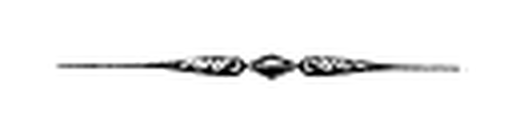
\includegraphics[width=0.23\linewidth]{assets/PA20_final_ornament_presentation_4x.png}
\end{center}

\end{document}
